%!TEX root = paper.tex
\section{\bluetana: Searching for Stealthy Skimmers with Smartphones}
\label{sec:tool}

In this section we describe the information we were able to retrieve from the
Bluetooth environment via Bluetana, an Android app we created and crowdsourced
to investigators.
%
We demonstrate how this information can be used to isolate potential skimmers
and the forensic limitations on data collection.

% In order to work on the detection and prevention of skimming due to internally
% installed devices, the features of the devices which are visible to an observer
% must be described. Without specialized hardware, the data which is collectable
% about an internal skimmer is that which is exposed through the device's
% Bluetooth interface \footnote{In this section, we address those portions of the
% Bluetooth interface which are exposed while the device is in
% \textit{discoverable} mode. Challenges and possibilities for handling
% non-discoverable mode are addressed in the discussion}. This interface includes
% inquiry response metadata from the device, serial port profiles (SPP)
% accessible following initial connection, physical layer data such as signal
% strength and location of observer, and possibly information which could be
% exfiltrated by initiating a serial connection with the device and sending
% commands or fuzzing input.

\subsection{Finding Bluetooth Modules with Scans} %{{{

 

\subsubsection{Limitation: Only scanning, no connecting} %{{{
\label{sec:cant-connect}

While some information on whether a device is a skimmer or not could be gleaned
from connecting to the device and attempting to send it commands, this would
interfere with forensic evidence.
%
The firmware on some skimmer modules records the last paired MAC address.

This inability to pair creates further inconvience in our crowdsourced approach.
%
Bluetooth provides the ability to query the services that a device can provide
without establishing a connection to the device, the Service Discovery Protocol
(SDP).
%
However, as of Android 6.0 the \texttt{BluetoothDevice} method
\texttt{fetchUuidsWithSdp} will automatically trigger a pairing process with the
device, making skimmer fingerprinting via SDP infeasible.
 

% \noteby{MB}{The below section should be cut down: just say that SDP profiling
%   is a no go, no need to get all nitty-gritty}
% The primary challenge in using a smartphone to detect skimmers is, we are
% limited to the data we can obtain from innocuous Bluetooth scans.
% %
% This is particularly a problem at fuel stations, where Bluetooth scans are
% likely to return legitimate devices; from auto entertainment systems, to service
% station equipment.
%  
% As such, one way to conclusively detect a skimmer would be to see if something
% is a skimmer by establishing a Bluetooth connection to it to get as much
% information about the type of Bluetooth device, and even sending it commands
% that skimmers are known to respond to, to see if it responds in the same way
% that known skimmers do.
% %
% This is what the SparkFun Skimmer searching app does with all default name HC
% devices that it discovers.
%  
% This practice may seem harmless, but our discussions with law enforcement
% reveals that this to be harmful to future investigations.
% %
% The reason is, the firmware in the HC modules record the last paired MAC address
% \todo{command?}.
%  
% This restriction has other consequences.
% %
% Bluetooth provides the ability to query the services that a device can provide
% without establishing a connection to the device, the Service Discovery Protocol
% (SDP).
% %
% This could be helpful for finding skimmers, as prior work has shown that SDP can
% be used to fingerprint bluetooth devices \cite{herfurt2004remote}.
% %
% Unfortunately as of Android 6.0, the \texttt{BluetoothDevice} method
% \texttt{fetchUuidsWithSdp} will automatically trigger a pairing process with the
% device, making this kind of fingerprinting infeasible.
%  
% The Linux Bluetooth stack (BlueZ) does not require paring to list the services
% that Bluetooth provides \todo{cite}.
% %
% In BlueZ you can run \textit{SDPtool} that for some specific bluetooth dongles
% it can list the profiles without connecting.
% %
% In fact, in the Bluetooth spec it says that you can list the \noteby{MB}{Maybe
% we can take this out, or push it into the future work section, or note that the
% above belongs to future work? I don't feel like it is neccessary here} %}}}


%
% \subsection{Implementation} 
% In order to see whether these features could lead to skimmer detections, we
% engineered an application for data collection, codenamed ``Bluetana'' (Blue
% Katana), which runs on Android and records Bluetooth scan data, uploading
% everything it sees to a database on a regular basis.
%
% The app flags devices sharing a OUI with typical skimmer modules as red, to
% indicate to the user that performing localization of the device will aid in the
% detection process.
%
% The application records a timestamp, a location of the observer device when an
% enquery-response packet is recieved, a confidence interval for that geolocation,
% the MAC of the device seen, signal strength, the observer's MAC, the name
% received from the enquery-response, if any, whether the device is Classic, LE,
% or Both, as well as the device class.

% Once a certain number of responses have been recorded by the app(3KB), a CSV of
% all the inquiry responses is uploaded automatically to a database for further
% analysis. The data is then used to generate real time statistics and maps of the
% scanned gas station investigated. This is paired with a web application that
% allows searching records by generic criteria, and heatmaps of the clusters of
% geolocations of observers when they receive enquiry response packets, allowing
% easy visual localization. The system also notifies the group whenever a skimmer
% match a high number of criteria is seen, allowing us to inform our partners in
% the field to perform a thorough investigation.

%

\if 0 % extra text {{{ From the government inspectors we worked with, a
reverse-engineering of other skimmer-detection apps, searching through skimmer
``for sale'' sites on wordpress, facebook, and tor, and articles online, we
developed ideas of what an internal skimmer module would look like. Reports of
recovered skimmers in Arizona and elsewhere inform us that there are only a
handful of bluetooth modules used by criminals.

\subsection{Characteristics of Bluetooth devices at gas stations}

To identify characteristics that can help in Bluetooth skimmer detection, we
performed an exhaustive initial survery of gas of 1000+ gas stations, spread
across various counties in Maryland, California, Illinois and Nevada. For the
survey, we setup a simple Android app to continuously perform discovery
requests, and record all response packets received, alongwith timestamp and
geolocation to a remote database. There exist apps for performing MAC address
based detection of skimmer modules, but none which allowed for data collection
at scale. Working from our data, we were able to identify skimmer features more
powerful than MAC-based filtering, and develop a high accuracy picture of the
Bluetooth environment at gas stations.

\begin{itemize}
    \item \textbf{Bluetooth type} : It is typical to see a large number of
Bluetooth devices at gas stations. We analyzed the number of Bluetooth devices
seen at a gas station, and also break them down by device type - LE and classic.

	\begin{figure}[h] \centering
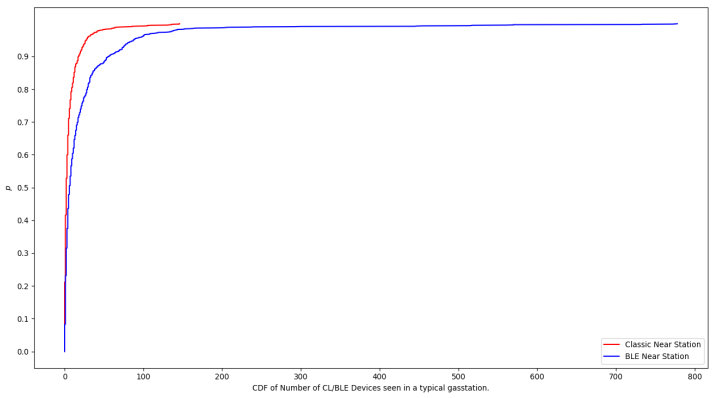
\includegraphics[width=1\columnwidth]{fig/cdfs_classic_ble.png}
  	\caption{CDF of classic vs LE devices seen near gas
stations. \textit{Classic Bluetooth devices are far less common in the vicinity
of a gas station than LE devices}}
  	\label{fig:cdf_classic_le}
	\end{figure}

	From the graph, it can be seen that that while there maybe a large
number of Bluetooth devices in the proximity of a gas station area, typical
number of classic devices is significantly lower than LE devices. From reports
of previously recovered skimmers, it is known that classic Bluetooth serial
modules are the most popular use in skimmers. The key insight here therefore
being that while there are a large number of Bluetooth devices seen at a gas
station, the number of applications using classic Bluetooth modules are far
fewer, and thus device type can be used as a filtering mechanism when looking
for skimmers.
	\item \textbf{MAC address and manufacturers}: Bluetooth MAC addresses
are 48 bit in length and follow the IEEE 802 MAC address conventions. According
to this, the first 24 bits of the address are an Organization Unique Identifier
(OUI), which identify the manufacturer of the Bluetooth module. The list of all
OUIs are maintained are publically available and maintained by the
IEEE. \todo{insert figure of first three bytes OUI}

	It is therefore possible to identify the manufacturer of a particular
device. Because it is known that skimmers are armed with commodity Bluetooth
serial modules manufactured by a certain number of manufacturers, the key
insight here is that the OUI can be used to identify whether an observed module
is from one of these manufacturers.

	\item \textbf{Class of Device}: The class of device field in a discovery
response packet indicates the kind of end user applications/services that the
Bluetooth device supports. The device class is split into two segments - major
and minor device class. The major device class indicates the high level
functionality of the device, whereas the minor device class indicates the
specific kind of device with respect to the high level functionality. For
example, a typical smart phone will have a major device class of 'Phone', and
minor device class of 'Smart phone'.  \\ Of particular interest here is the
major device class - 'Uncategorized: device code not specified'. This indicates
that a particular Bluetooth device doesnt have an end application defined or the
application will be defined later. This is the default category used by
Bluetooth chip and module manufacturers, with the responsibility of assigning
device class on the end equipment producer. A key insight therefore is that a
device responding with an uncategorized CoD is hightly likely to be a prototyped
board using a typical Bluetooth module, which fits, amongst others the
description of a skimmer.

	\item \textbf{Bluetooth Name}: Using string edit distance (Jaro-Winkler)
clustering, with a scaled cluster distance cutoff point as the size of our data
grew, we were able to accurately flag ``odd device names'' after filtering from
other mechanisms, such as the MAC address and class of device had been
performed. This has two benefits to the search for skimmers. One, it is a highly
accurate manner by which to detect that a skimmer exists. The likelihood of
someone buying a commodity bluetooth module that is not sold as a product and
taking the time to rename it then plant it in a gas station \textit{without it
being a skimmer} is assumed to be quite low, if not non-existent. Thus, if we
see an oddly named device as flagged by the clustering, we have high confidence
that it is a skimmer. Second, it gives us an idea of which devices are not
likely to be skimmers. For instance, there are devices named ``AP-*''
\footnote{The star indicates one or more characters. In this case, the portion
of the name is a series of seemingly random hexadecimal digits.}, are all
clustered together, and devices named in this way typically correspond to
Bluetooth Onboard-Diagnostics Scanners used at smog check businesses. These
devices use the same modules as are commonly found in skimmers. Using a naive
approach, we might flag this device as a skimmer, but as a result of knowing the
frequency of this device name, when one of these devices is notified to us via
the application pipeline for finding skimmers, we may look more carefully into
the localizaiton, and more easily determine whether or not it actually is a
skimmer.
\end {itemize}

The above Bluetooth descriptors can be used to detect presence of skimmers at a
gas station. In the next section we introduce the design of Bluetana, that
leverages these characteristics.

\subsection {Bluetana Design} With the goal of designing a crowd-sourced,
scalable detection mechanism for skimmers, we designed the Bluetana toolkit. The
toolkit toolkit performs detection by performing Bluetooth scanning, filtering
responses on the basis of two lists that define commodity Bluetooth serial
modules. The two lists are described as below :

\begin{enumerate}
\item \textbf{Hitlist: } We define a list of possible skimmer modules (referred
to henceforth as the \textbf{hitlist}). As discussed in in the previous
subsection, the first three bytes of the Bluetooth address reveal the
manufacturer of the device/module. Taking this into consideration, we build a
list of commodity Bluetooth serial module manufacturers. The hitlist contains 3
byte MAC addresses, from modules used in skimmers recovered in the field by law
enforcement agencies. We also include MAC prefixes of commonly available
Bluetooth-serial modules drawn in online marketplaces (such as ebay, Amazon,
Aliexpress, Sparkfun, Adafruit, Mouser, Digikey etc.). This hitlist is used
primarily to isolate suspicious modules from the myriad of modules observed
while scanning.

\item \textbf{Whitelist: } While the hitlist defines commodity modules commonly
used in skimmers, it is possible that the modules may be used for legitimate
purposes. A common occurence is of commercial OBD scanners which are typically
found at gas stations (mainly those which also have a smog check facility
on-site). Table \ref{tab:OBDvSkimmer} highlights an example

\begin{center}
\begin{tabu} to 0.8\columnwidth { | X[l] | X[c] | } \hline \textbf{Bluetooth
name} & \textbf{MAC Address} \\ \hline RNBT-D6E1 & 00:06:66:DA:D6:E1 \\ \hline
AP000888-1BB0 & 00:06:66:61:1B:B0\\ \hline
\end{tabu}
\label{tab:OBDvSkimmer}
\end{center}

The first row lists a device used in a recovered skimmer, whereas the second
device is used in an OBD skimmer. Since both use the same make Bluetooth module
(i.e., have same MAC prefix), the hitlist will flag both the devices. To resolve
this issue, we create a list of default device names, that use modules from the
hitlist but are known to be non-skimmer legit devices. This is called as the
whitelist, and has been generated from our crowd-sourced data collected as
described in the previous section
\end{enumerate}

The lists defined above are used by the two key components of our toolkit - a
front-end app for Bluetooth data collection, and a back-end database to store
and perform analysis on the data. Additionally we also define a hitlist of
commonly known Bluetooth skimmer modules to identify suspicious devices. The
toolkit components are detailed as follows:

\begin{enumerate}
\item \textbf{Front end Android app: } The front-end application was developed
as a method of crowdsourced data collection on the Bluetooth environment, as
well as a medium for real-time detection of skimmers. The application, which can
run on standard consumer-grade cell phones (running API level 21 or Android 5.0
and above), works by performing continuous inquiry scans and recording the
responses recieved. The app allows for variable scan timing, ranging between 1
second and a full scan (\textasciitilde23 seconds)[\todo{decide whether we wanna
discuss scan time choices, maybe here or in discussion}]

As the app receives Bluetooth device information from inquiry scans, it displays
them on the app UI in real time. For each device, we display the Bluetooth
address, Bluetooth device name, RSSI and class of device. If a device MAC
address matches any entry on the hitlist, it is highlighted in red. For devices
flagged by the hitlist, if the device name matches an entry on the whitelist or
the device class is not 'Uncategorized', it is instead highlighted in
orange. This color coding of devices, reflects the threat level of a particular
device (red - highly suspicious, orange - possibly suspicious). Additionally the
RSSI can be used in real time to localize a particular device to a specific
location within the confines of a gas station. These features enable the app to
be used for real time detection and tracking of skimmer devices by the
investigator.

\item \textbf{Back-end Database} Once a certain number of responses have been
recorded by the app(3KB), a CSV of all the inquiry responses is uploaded
automatically to our back-end database. The back-end database is hosted on a
secure,remote storage server located at our end. The records are stored in a
Postgresql (PSQL) database for further analysis. At the back-end the data is
then used to incrementally improve the accuracy of the hitlist and whitelist,
and also to generate real time statistics and maps of the scanned gas station
investigated. The back end system also contains configured alarms to notify
whenever a possible skimmer is flagged, allowing us to inform our partners in
the field to perform a thorough investigation.
\end{enumerate}

We were unable to legitimately deploy this crowdsourced approach to hundreds of
individuals due to a restriction in the trusted computing base for skimmer
detection: law enforcement and the weights and measures departments at the state
level. In lieu of being able to deploy the application to the google play store,
we opted to perform a survey of every at-risk gas station in one metropolitan
area. This consisted of over 200 hundred unique individual stations; the
experimental design of this survey is detailed below.  \fi %}}}
